%!TEX program = xelatex
% 完整编译: xelatex -> biber/bibtex -> xelatex -> xelatex
\documentclass[lang=cn,a4paper,newtx]{elegantpaper}

\title{操作系统:实验大作业}
\author{王天一 \\ 320200931301}

\date{\zhtoday}
\usepackage{array}
\newcommand{\ccr}[1]{\makecell{{\color{#1}\rule{1cm}{1cm}}}}
\addbibresource[location=local]{reference.bib} % 参考文献,不要删除

\begin{document}

\maketitle


% 提交内容需包括:
% 1实验报告
% 实验目的
% 实验方法及过程(关键数据结构与算法,可以给出流程图等伪代码描述)
% 执行结果及分析(包括执行截图截图)
% 2源码压缩包

\section{实验内容}
\begin{itemize}
    \item \textbf{进程间通信}:Linux环境下编写一个C语言程序,读取一个数据文件(自定义一个大的整数文件),对每一个数据进行某种运算,再在屏幕输出计算结果。要求以上工作用3个进程实现,进程1负责读文件,进程2进行计算,进程3负责将计算结果输出到文件result.txt中。进程间通信分别使用管道、共享内存机制,并比较不同方式的时间性能。
    \item \textbf{内存管理}:Linux下编写一个程序,利用内存映象文件,实现less工具的功能(多屏显示)
\end{itemize}
\section{实验环境}
本次实验使用的环境为一台装有Ubuntu Server 22.04.2 LTS操作系统的机器。其中配置如\figref{fig:neofetch}所示。
\begin{figure}[!htb]
    \centering
    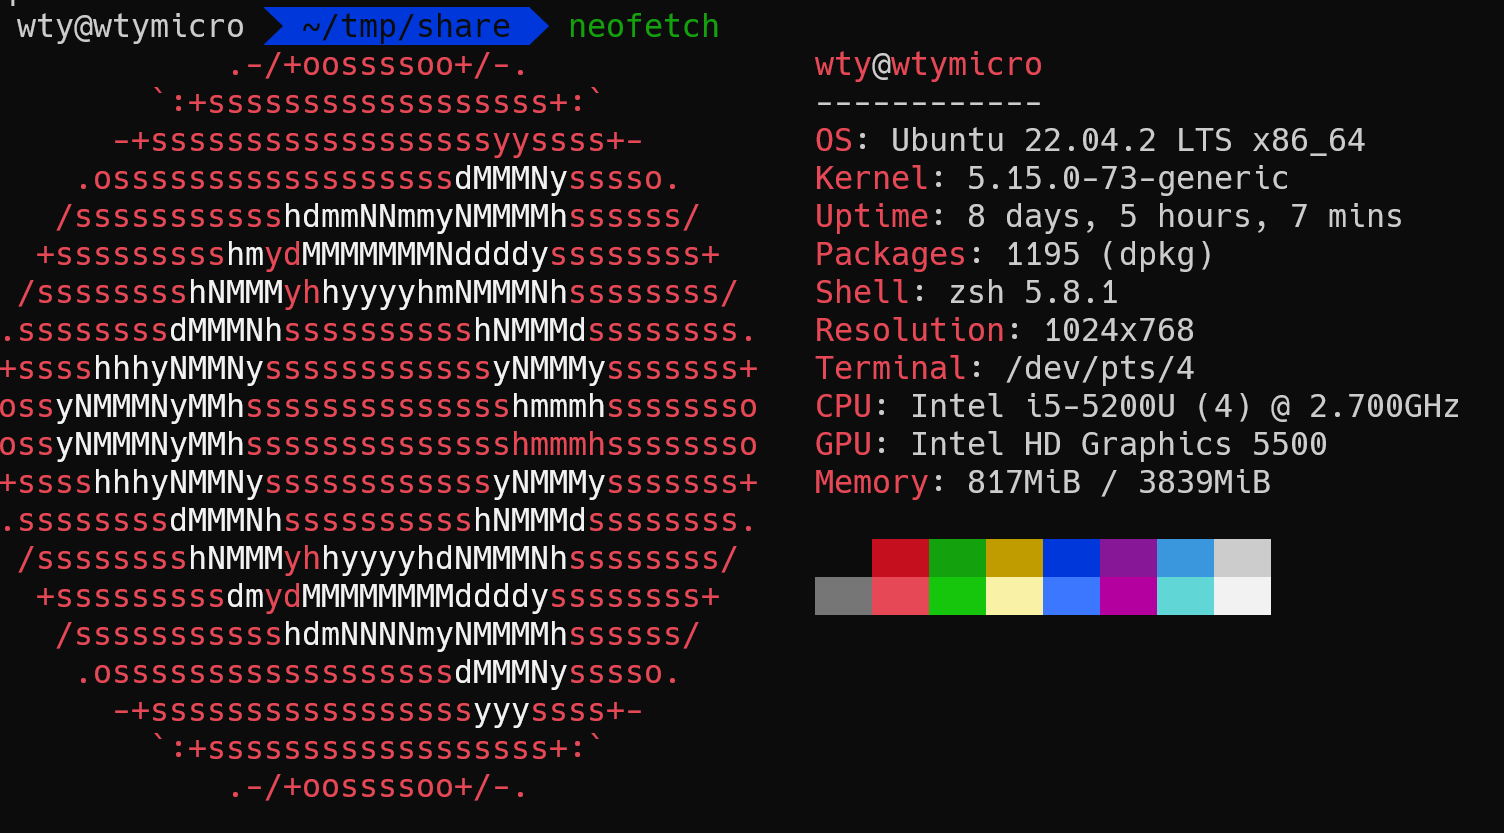
\includegraphics[width=0.7\textwidth]{image/neofetch.png}
    \caption{实验设备配置}
    \label{fig:neofetch}
\end{figure}

\textbf{注:}为了确保实验环境的准确性,实验中的数据均使用\verb|taskset|命令进行绑定核心的操作,故可以去除机器核心数对结果的影响。
\section{算法设计}
\subsection{进程间通信}
对于进程间通信,我们需要设计我们的程序,使用三个进程实现以下工作:
\begin{itemize}
    \item 进程一读取本地的文件,将读取出来的数据通过某种进程间通信手段传输给进程二。
    \item 进程二接收进程一发送的数据,进行某种运算(这里我们选择对214取模),并将结果发送给进程三。
    \item 进程三接收进程二发送的数据,将其写入结果的文件中。
\end{itemize}

\subsubsection{基于管道的实现}


管道(pipe)是一种常用的进程间通信(IPC)机制,用于在两个相关进程之间传输数据。它提供了一种简单的单向通信方式,其中一个进程充当写入数据的发送者,而另一个进程则充当接收数据的接收者。在本次实验中我使用Linux提供的\verb|pipe()|函数来创建进程之间的匿名管道来进行进程间通信。


\subsubsection{基于共享内存的实现}

共享内存是一种进程间通信的高效方式,它允许多个进程共享同一块内存区域,从而避免了数据复制和操作系统内核的介入。本次实验中,我使用了\verb|shmget|创建进程中的共享内存,并使用信号量机制对共享内存这一临界资源进行管理,保证其运行的正确性。

\subsection{自制less工具}

less 是一个功能强大的用于浏览文本文件的命令行工具。它可以在终端中按页显示文件内容,并提供了很多方便的导航和搜索功能。本次实验中我主要实现了less的以下几个功能:
\begin{itemize}
    \item \textbf{分屏浏览}:一屏一屏的加载数据,避免全部加载数据导致的卡顿。
    \item \textbf{自适应窗口}:根据当前终端的高度自动调成程序的输出,保证程序可以一直占满整个终端。
    \item \textbf{禁用缓冲}:在运行的过程中禁用终端的输入缓冲区,实现按下某个按键程序可以直接相应的效果,而不是需要按下回车才会有反应。
    \item \textbf{分行移动}:可以一行一行的向前或者向后移动屏幕。
\end{itemize}

\subsubsection{分屏浏览}

分屏浏览的功能实现核心思路是对mmap内存映射函数的使用。在程序的开始,我们需要先将文件从硬盘映射到内存中,将文件映射成一个字符数组。

然后根据要进行的不同的操作,使用memcpy函数将文件中的内容拷贝到缓冲区,最后使用printf函数将缓冲区的内容打印到终端上。
\subsubsection{自适应窗口}
为了获取终端窗口的大小,我使用\verb|termios.h|头文件提供的\verb|ioctl|函数动态获取当前终端的高度,并将其赋值给一个全局变量,其他的函数通过此全局变量的值来调节其输出的高度。
\subsubsection{禁用缓冲}
为了禁用输入缓冲区,我使用\verb|termios.h|头文件提供的\verb|tcsetattr|函数动态设置当前终端属性,禁用标准模式和回显,实现禁用输入缓冲区的功能。
\subsubsection{分行移动}
为了实现分行移动,我添加了两个分支,分别是j和k(对应vim的键位),当按下j时,会向下移动一行,当按下k时,会向上移动一行。
\section{实验过程}
\subsection{进程间通信}

我使用Python编写了一个脚本\verb|gen_data.py|,生成了一百万个整数,其大小为6.9兆字节,我们以此作为实验的测试数据。脚本的核心循环如下所示:
\begin{lstlisting}[language=python]
    def gen_data():
    # 生成1到1000的数据
    with open('testdata.txt', 'w') as f:
        for i in range(1, 1000001):
            f.write(str(i) + '\n')
\end{lstlisting}

我使用如\tabref{table:com_env}所示的环境对我自己的程序进行性能分析。
\begin{table}[htbp]
\centering
\caption{测试过程中的各种选项}
\label{table:com_env}
\begin{tabular}{cc}
\hline
\textbf{参数} & \textbf{数值}           \\ \hline
Make版本      & 4.3                   \\
gcc 版本      & 11.3.0                \\
编译选项        & -O3(未附加-g符号表)         \\
计时方法        & timeval(精度到微妙)        \\
编写方式        & 所有函数均没进行特殊处理(static inline、Likely等优化手段) \\ \hline
\end{tabular}

\end{table}

为了保证实验结果的可靠性,我们编译完程序源代码后,使用taskset命令将其锁到一个核心上运行五次,取其运行时间的平均值,最后两种方案的平均值如\tabref{table:res}所示。
% 实验结果
% time cost:8.093155s
% taskset 01 ./out  2.52s user 5.57s system 99% cpu 8.095 total
% time cost:7.985894s
% taskset 01 ./out  2.51s user 5.47s system 99% cpu 7.988 total
% time cost:8.019982s
% taskset 01 ./out  2.47s user 5.55s system 99% cpu 8.022 total
% time cost:7.972469s
% taskset 01 ./out  2.46s user 5.51s system 99% cpu 7.975 total
% time cost:8.008781s
% taskset 01 ./out  2.42s user 5.59s system 99% cpu 8.011 total


% time cost:0.234102s
% taskset 01 ./out  0.22s user 0.01s system 99% cpu 0.237 total
% time cost:0.239479s
% taskset 01 ./out  0.23s user 0.01s system 99% cpu 0.242 total
% time cost:0.215798s
% taskset 01 ./out  0.21s user 0.01s system 99% cpu 0.218 total
% time cost:0.247622s
% taskset 01 ./out  0.25s user 0.00s system 99% cpu 0.250 total
% time cost:0.228334s
% taskset 01 ./out  0.22s user 0.01s system 99% cpu 0.231 total

\begin{table}[htbp]
\centering
\caption{实验结果}
\label{table:res}
\begin{tabular}{ccccccc}
\hline
\textbf{实现方法} & \textbf{第一次实验} & \textbf{第二次实验} & \textbf{第三次实验} & \textbf{第四次实验} & \textbf{第五次实验} & \textbf{均值} \\ \hline
\textbf{管道}   & 8.093155s      & 7.985894s      & 8.019982s      & 7.972469s      & 8.008781s      &  \textbf{8.0160562s}           \\
\textbf{共享内存} & 0.234102s      & 0.239479s      & 0.215798s      & 0.247622s      & 0.228334s      &\textbf{0.233067s}             \\ \hline
\end{tabular}

\end{table}

通过结果可以看出,共享内存的结果远优于管道,这里我猜测是由于使用pipe()导致了过多的陷入(trap)导致浪费很多时间,所以我又使用了Linux下的\verb|time|命令测试内核态和用户态花费的时间,其结果如\tabref{table:res_time}所示,可以看到在使用管道的程序中,内核态花费了大量时间(69\%),但在共享内存的程序中,内核态只花费了很少的时间(3\%),符合我们的猜测。
\begin{figure}[!htb]
    \centering
    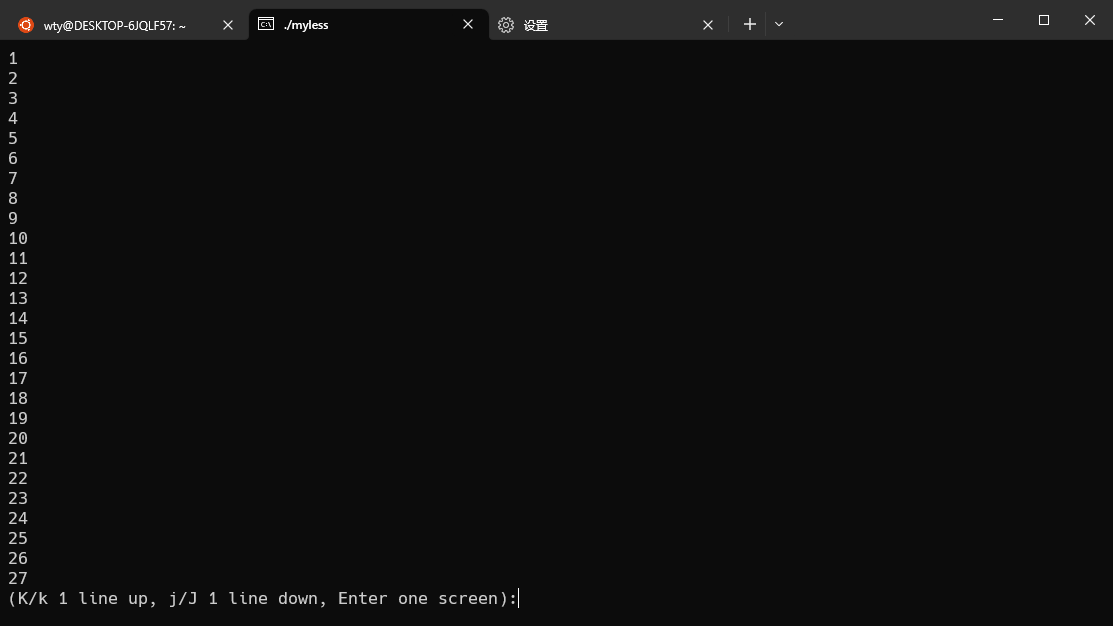
\includegraphics[width=0.7\textwidth]{image/less_open.png}
    \caption{自制less工具打开文件}
    \label{fig:less_open}
\end{figure}
\begin{figure}[!htb]
    \centering
    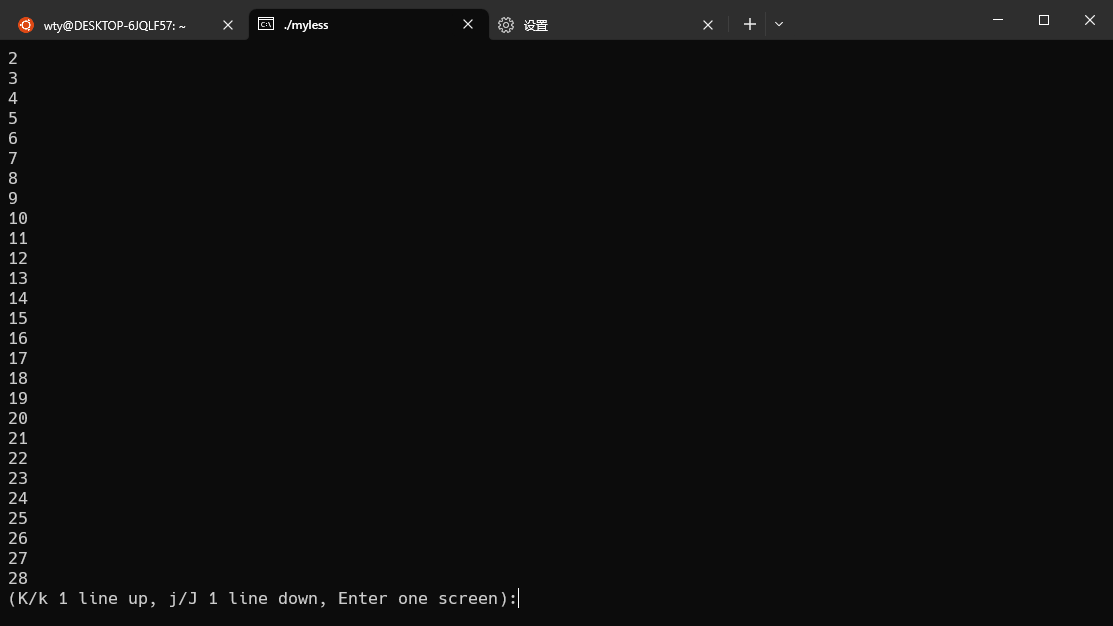
\includegraphics[width=0.7\textwidth]{image/less_j.png}
    \caption{自制less工具向下移动一行}
    \label{fig:less_j}
\end{figure}
\begin{figure}[!htb]
    \centering
    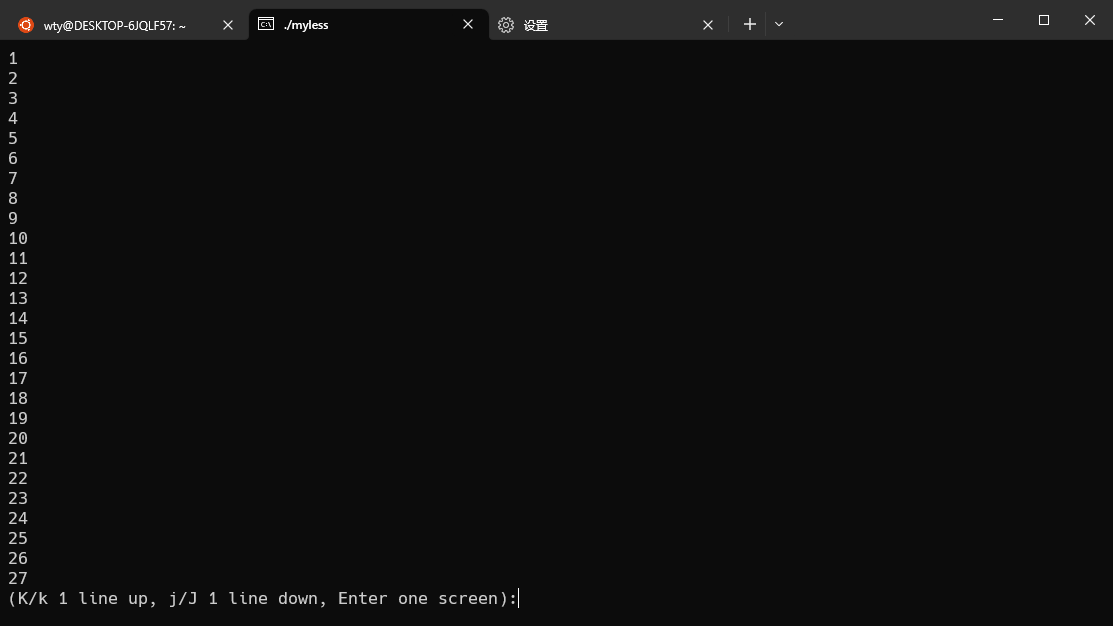
\includegraphics[width=0.7\textwidth]{image/less_k.png}
    \caption{自制less工具向上移动一行}
    \label{fig:less_k}
\end{figure}
\begin{figure}[!htb]
    \centering
    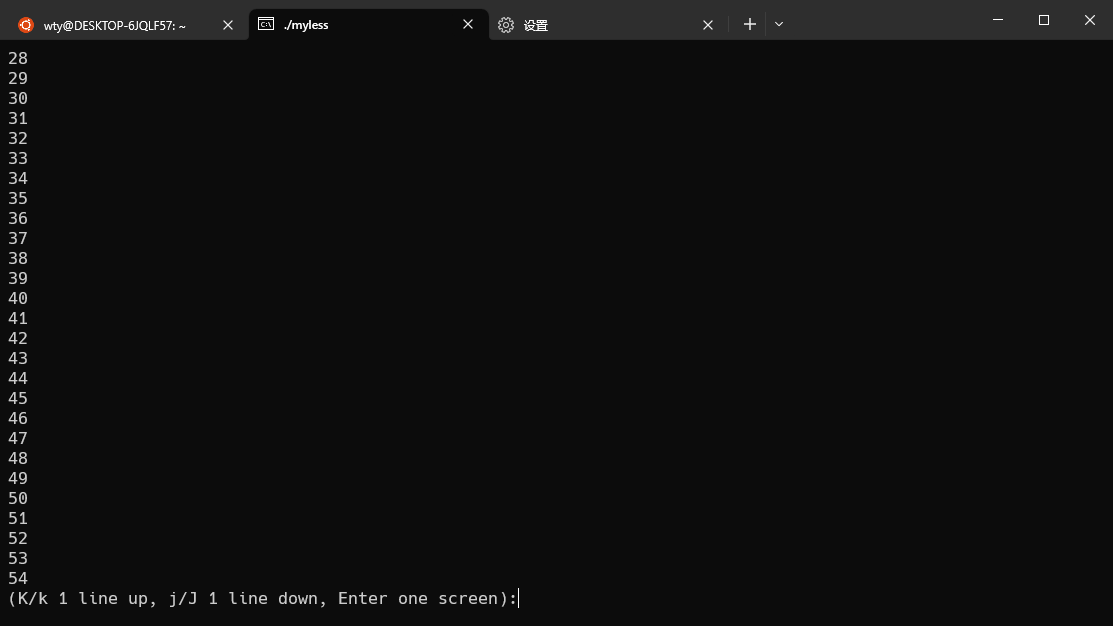
\includegraphics[width=0.7\textwidth]{image/less_enter.png}
    \caption{自制less工具向后翻一整页}
    \label{fig:less_enter}
\end{figure}
\begin{figure}[!htb]
    \centering
    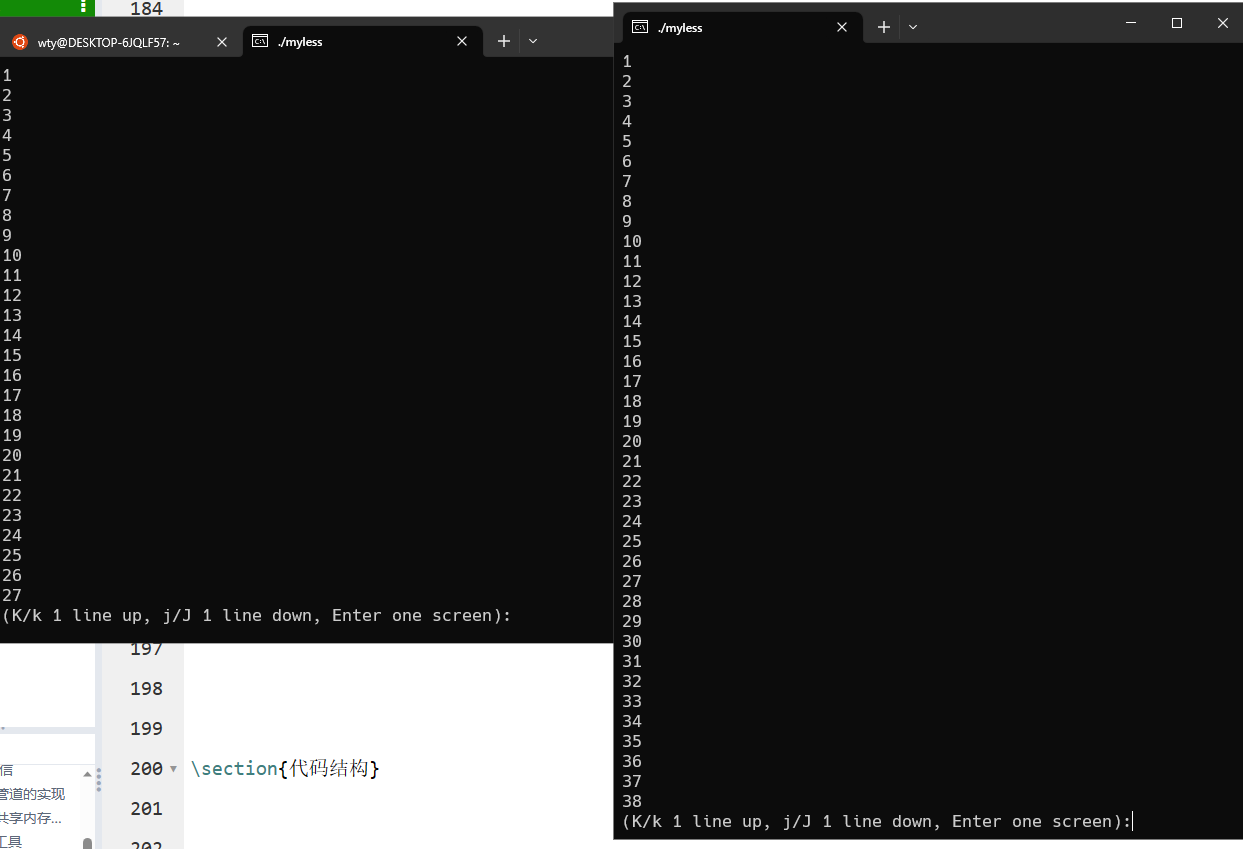
\includegraphics[width=0.7\textwidth]{image/less_diff_height.png}
    \caption{自制less工具自适应高度}
    \label{fig:less_diff_height}
\end{figure}
\begin{table}[htbp]
\caption{time测试实验结果(五次均值)}
\label{table:res_time}
\centering
\begin{tabular}{ccccc}
\hline
\textbf{实现方法} & \textbf{用户态时间} & \textbf{用户态占百分比} & \textbf{内核态时间} & \textbf{内核态占百分比} \\ \hline
\textbf{管道}   & 2.476s         & 30.9\%            & 5.538s         & 69.1\%            \\
\textbf{共享内存} & 0.226s         & 97.0\%            & 0.008          & 3.0\%             \\ \hline
\end{tabular}
\end{table}

结合上面的实验和猜测,我们可以分析出管道的效率低下是反复陷入内核造成的。

\subsection{自制less工具}

在进行完进程间通信的试验后,我们可以直接使用其生成的文件作为测试文件来测试我们自制less工具的性能。首先是最基本的打开文件,其命令如下所示,结果如\figref{fig:less_open}所示,可以看出打开文件的功能正常。
\begin{lstlisting}[language=bash]
    ./myless ../shared_mem.txt
\end{lstlisting}

然后测试其翻页功能,首先我们按下j键,测试其向下移动一页的功能,结果如\figref{fig:less_j}所示,可以看出整个窗口显示的数据向下移动了一行,然后再按下k键向上移动一行,结果如\figref{fig:less_k}所示,可以看出整个窗口显示的数据向下移动了一行,说明翻页功能正常。

再按下回车翻一整页,结果如\figref{fig:less_enter}所示,可以看出的确移动了一整页。说明翻一整页的功能也正常。

最后再测试自适应功能,打开两个终端连接机器的ssh,然后以不同的高度打开自制less工具,如\figref{fig:less_diff_height}所示,可以看到在不同高度下,程序均能占满整个终端。

\section{代码结构}

本次作业的代码结构如下:
\begin{itemize}
    \item \textbf{data}:包含生成测试数据的Python脚本和生成好的测试数据。
    \item \textbf{less}:包含自制less文件的源代码和Makefile文件,以及在X86平台上编译好的二进制可执行文件。
    \item \textbf{pipe}:包含使用管道实现实验第一部分的所有源代码和Makefile文件,以及在X86平台上编译好的二进制可执行文件。
    \item \textbf{result}:存储结果的文件夹,这里存放了我进行实验时候生成的数据。
    \item \textbf{shared\_memory}:包含使用共享内存实现实验第一部分的所有源代码和Makefile文件,以及在X86平台上编译好的二进制可执行文件。
    \item  \textbf{report}:包含报告的所有tex源代码文件和编译好的PDF版本,如果需要从源码构建,请使用xelatex编译链进行编译。
\end{itemize}

注:本次作业的所有代码均已开源至\href{https://github.com/wtyqqq/OS_Assignment}{github},仓库内有详细的git提交记录可作为原创证据。
\section{执行结果及分析}

本次实验中我首先分别基于管道和共享内存的方法进行了进程间通信的实验。实验结果显示共享内存的性能远优于进程间通信。我们通过猜测河实验证明这是频繁的使用管道会导致过多的陷入内核,频繁的切换浪费了大量的时间。
% \bibliographystyle{unsrt}
% \nocite{*}
\printbibliography[heading=bibintoc, title=\ebibname,sorting=none]

\appendix
% \appendixpage
\addappheadtotoc

\end{document}
